\documentclass[UTF8]{ctexart}
\usepackage{geometry}
\geometry{left=3.18cm,right=3.18cm,top=2.54cm,bottom=2.54cm}
\usepackage{graphicx}
\usepackage{tikz}
\newcommand*{\circled}[1]{\lower.7ex\hbox{\tikz\draw (0pt, 0pt)%
    circle (.5em) node {\makebox[1em][c]{\small #1}};}}
\usepackage{hyperref}
\hypersetup{
colorlinks=true,
linkcolor=black
}
\pagestyle{plain}	
% \usepackage{booktabs}
% \usepackage{subfigure}
\usepackage{setspace}
\date{}

\usepackage{ctex}
\usepackage{amsmath}

\renewcommand{\baselinestretch}{1.5}
\begin{document}
\ttfamily \songti
\zihao {-4}

\begin{center}
    \quad \\
    \quad \\
    \heiti \fontsize{45}{17} 研\quad 究\quad 报\quad 告
    \vskip 3.5cm
    \heiti \zihao{2} 通过分析慕测平台数据分析学生编程能力	
\end{center}
\vskip 3.5cm

\begin{quotation}
    \songti \fontsize{15}{15}
    \doublespacing
    \par\setlength\parindent{12em}
    \quad 

    学\hspace{0.61cm} 院:\underline{\quad 软件学院\quad}

    创建时间:\underline{2020年7月20日}

    学生姓名:\underline{戴俊浩,郭增嘉,刁苏阳}

    学\hspace{0.61cm}号:\underline{\small 181250022,1812500xx,181250026}

    教\hspace{0.61cm}师:\underline{\qquad 陈振宇 \qquad}
    \vskip 2cm
    \centering
    2020年07月21日
\end{quotation}

\newpage
\tableofcontents
\newpage
\section{研究问题:学生编程能力探究}
\subsection{详细介绍}
我们将研究方向设定为学生编程能力的分析,我们通过主成分分析法对平台的数据进行题目难度分析
然后结合分析的题目难度,将学生的编程得分等因素综合考量,使用相关性检测之后将高度重复的
变量除去,最后使用多元线性回归对高维数据进行分析,产生可视化的三维函数,得出一个学生的
编程能力的计算公式,当学生答题产生数据后就能通过相应的算法来得出这个学生的编程能力。
\subsection{研究背景}
在编程实践越来越热门的今天,网络上已有大量的OJ平台供用户练习。这些OJ平台之间的竞争是激烈的,
为了获取用户,平台必须在一系列重要指标上比别人做得更优秀。而评价OJ平台的重要指标之一,就在于
其能在有限的时间内帮用户最大化地提升能力。想要满足这个指标,避免让用户陷入盲目的题海战术,
这就需要平台能对题目的难度以及用户的编程能力有清楚到足以量化的认识。
\subsection{应用场景与价值}
我们现阶段的研究成果可以应用于网路上的在线编程平台,通过学生对题目的完成实践、提交次数、得分数量等
诸多维度外加对于学生代码的分析,归纳评判一个题目的难度以及一个学生的编程能力指标,尽可能展示一个学生
编程能力的真实水平。

在大数据平台的支持下,学生可以明确定位自己的编程能力,同时明晰题目的具体难度水平,从而选择适合自己
的题目进行锻炼,方便学生采取合适的学习路径,省却大量筛选题目的实践,有效提升编程能力和代码水平。
\section{研究方法}
\subsection{数据源}
使用了慕测平台的数据,分析学生的编程能力,通过OJ提供的json文件可以看到学生的userID以及一系列的提交记录,使用python读取json文件获取所需数据。
\subsection{数据分析}
\subsubsection{主成分分析}
在处理题目难度的时候使用了PCA\footnote{即主成分分析法,下文中全部使用主成分分析法},首先将题目的数据通过对json文件的分析导入到一个矩阵中,这个矩阵是一个3000*7的矩阵,7列是题目的7个维度的数据
,分别是该题的初始提交分,该题的最终得分,该题的平均分,该题的最终得分和提交次数的比值,该题的前一半的提交的斜率,也就是用户在做题时分数的增长
速率还有该题的总耗时以及该题的最终分数和其他题目的最终分数的差值。通过对json文件的读取实现了对这些数据的分析。

使用主成分分析法,首先将数据注入到3000*7的二维数组\footnote{3000是题目的数量,虽然实际上题目编号从200+开始,但是使用了全部题号,如果产生更多题目需扩容}
中,从7个维度展现这个题目难度c。将所有的数据减去该列的平均值。做标准化,然后将二维数组转换为矩阵,
求矩阵的协方差矩阵即$C=B^T \cdot B$,然后一次求出特征值和特征向量,对特征值进行排序,选取最大的一个特征值对应的列作为主成分,得到相应的投影矩阵,
最后利用投影矩阵得出降维之后的数据($E = B \cdot D^T$),最后对得到的数据进行标准化,将数据的区间限定为$[0,1]$,这样就使用主成分分析的方法
获得了题目的难度系数。
\subsubsection{相关性分析(pearson)与显著性检验}
在处理学生编程能力的多维数据时,我们意识到这多个维度之间可能具有高度的相关性。
我们对下列维度计算了其之间的pearson相关系数,分别是学生的得分(综合了最终得分与难度)、
学生的最初得分、学生的分次比、学生的总耗时、学生与该题平均值的差值、学生的规范分。

我们先把数据做标准化处理,然后注入一个6*271的矩阵\footnote{271是用户的总数}。在对这个数组
计算其pearson相关系数后,我们得到一个6*6的矩阵。这个矩阵的第i行第j列和第j行第i列的
值均表示原矩阵第i行与第j行之间的pearson相关系数。$$ r_{X,Y}=\dfrac{n\sum_{i} X_iY_i-\sum_{i} X_i \sum_{i} Y_i}{\sqrt{n\sum_{i} X_i^2-(\sum_{i} X_i)^2}\sqrt{n\sum_{i} Y_i^2-(\sum_{i} Y_i)^2}} $$
同时,我们也得到一个6*6的p-value矩阵\footnote{p-value是一种概率:在原假设为真的前提下,出现该样本或比该样本更极端的结果的概率之和。},
作为对pearson系数的显著性检验。

在最终确认高相关性的维度时,我们使用了相当严格的标准,要求pearson相关系数值大于0.9或小于-0.9,
p-value小于0.01。最后返回一个size为2的二维列表positive-negative,其中positive-negative[0]
代表高度正相关的维度对,positive-negative[1]代表高度负相关的维度对。
\subsubsection{多元线性回归}
处理学生的编程能力时使用了多元线性回归,我们尝试着将9位学生的样本的代码水平进行了评价,最后对他们的编程能力给出了一个分数,为了能够使多元线性回
归更加准确这9个学生是2个较差,5个一般和2个较好,多元线性回归中一共使用了4个变量对一个学生的编程能力进行分析,分别是学生提交的所有题目的平均分,
学生的提交分数和提交次数的比值,学生做这个题目所用的时间,学生的代码的规范得分。经过了上一步的皮尔森系数的相关性
检验这几个数据的相关性并不是特别大,所以将这些数据使用最小二乘法进行多元线性回归,得出了一个学生编程能力的计算公式,当学生产生了答题记录之后
就能通过OJ系统json数据大致估算出这个学生的编程能力。

首先将数据注入预设好的矩阵当中,每一行的第一项都是1,作为常数项的系数,将二维的数组转换为矩阵$X$,同时将我们对就为同学的评分注入到一个$9*1$的矩阵$Y$
中,之后使用\boldmath$$\hat{B}=\begin{pmatrix}
    \hat{b_0}\\\hat{b_1}\\\vdots\\\hat{b_p}
\end{pmatrix}=(X^TX)^{-1}X^TY$$\unboldmath
对数据进行计算就可以较为轻松的得出最后的学生的编程能力和几个数据之间的函数关系。
\subsubsection{数据可视化}
在多元线性回归之后,我们获得了各个维度对于结果的影响系数和偏移常量。
但高维度的函数更为抽象,我们难以根据单纯的数据判断此次多元线性回归的可信度和可行性。

我们抉择了其中影响最显著的两个维度(用户最终得分,分次比)作为元素绘制回归线进行可视化展示,
同时将各个学生的编程能力的相关系数一同绘制入可视化图中展现回归的具体效果和情况。

\begin{figure}[htb] 
\center{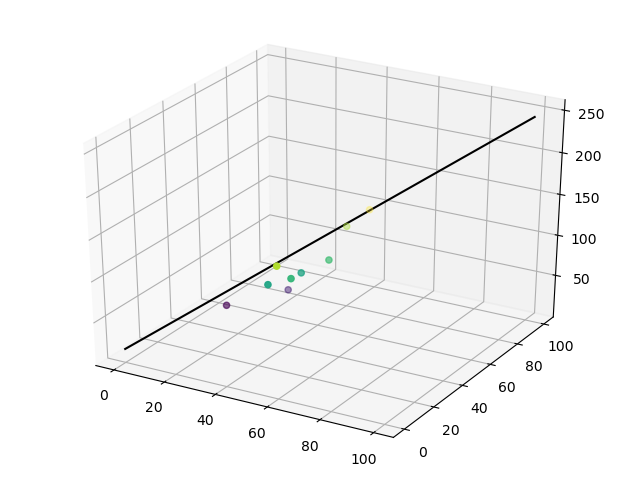
\includegraphics[width=5cm]  {myplot.png}} 
\caption{\label{1} 可视化} 
\end{figure}

从上图我们可以看到,代表各个学生编程能力的点围绕在回归线附近。
由此,初步判断以此多元线性回归所得学生编程能力分析函数的。(进一步确认需要更多信息以及数据的支持)
\section{代码解析}
\subsection{代码逻辑}
\subsubsection{题目难度分析模块}
题目难度部分一共有9个文件,其中包括了7个模块数据python处理文件,1个标准化函数,1个PCA算法。7个模块的数据读取和标准化函数都在component文件夹中。

\begin{enumerate}

    \item 文件夹中的averageScore.py读取了的caseid对应的所有用户的所有的提交分的平均值,并使用字典的形式进行了存储。
    \item 文件夹中的CompareTo.py读取了caseid对应的与其他题目的最终得分的平均分的差值,并使用字典的形式进行了存储。
    \item 文件夹中的FinalScore.py读取了caseid对应的所有用户最终得分的平均分,并使用字典的形式进行了存储。
    \item 文件夹中的FirstGit.py读取了caseid对应的所有用户的初始提交分的平均分,并使用字典的形式进行了存储。
    \item 文件夹中的FractionRatio.py读取了caseid对应的所有用户最终得分和用户所有的提交次数的比值,并使用字典的形式进行了存储。
    \item 文件夹中的HalfSlope.py读取了caseid对应的所有用户的前一半的提交和分数的斜率,并使用字典的形式进行了存储。
    \item 文件夹中的timeToSolve.py读取了caseid对应的所有用户的做一道题的总耗时的平均值,并使用字典的形式进行了存储。
    \item 最后有一个normalize.py文件可以接受一个字典,然后将字典中的所有的值做标准化,转换成[0,100]区间的值。

\end{enumerate}
最后在Usercomponent文件夹中使用了difficultMain.py引用了所有的上述模块,使用主成分分析法分析了数据,算出了最后的题目难度的值
\subsubsection{学生编程能力分析模块}

学生编程能力部分一共有10个文件,其中包括了6个模块数据python处理文件,1个标准化函数,1个pearson值与显著检验文件,
1个多元线性回归文件,1个pylint.conf文件。6个模块的数据读取和pylint.conf都在Usercomponent文件夹中。

\begin{enumerate}

    \item 文件夹中的userScore.py读取了的userid对应的所有题目的所有的最终得分*难度的平均值,并使用字典的形式进行了存储。
    \item 文件夹中的CompareToAverage.py读取了userid最终得分与本题平均得分的差值的平均值,并使用字典的形式进行了存储。
    \item 文件夹中的FirstUpload.py读取了userid对应的所有题目的初始提交分的平均分,并使用字典的形式进行了存储。
    \item 文件夹中的Fraction.py读取了userid对应的所有题目每次提交分之和和题目所有的提交次数的比值,并使用字典的形式进行了存储。
    \item 文件夹中的CodingStyle.py读取了userid对应的所有题目的规范分,并使用字典的形式进行了存储。
    \item 文件夹中的Time.py读取了userid对应的所有题目的耗时的平均值,并使用字典的形式进行了存储。
    \item 文件夹中的pylint.conf为CodingStyle使用的pylint的配置文件。

\end{enumerate}

在Component文件夹中使用了normalize.py接受一个字典,然后将字典中的所有的值做标准化,转换成[0,100]区间的值。
在dataSolve文件夹中使用Pearson.py引用上述所有模块计算pearson相关系数与p值,返回高度正和负相关的列表。
在dataSolve文件夹中使用MultiLinear.py进行多元线性回归,返回学生编程能力的值。
\subsubsection{数据可视化}
数据可视化技术依托于python的numpy及matplotlib.pyplot包。降序排列、筛选多元线性回归分析所获得的
各维度对最终成绩的影响程度,获得两个影响最为显著的维度,绘制多元线性回归线。同时,将对学生的维度分析数据
导入图标当中共同展示,从而直观分析多元线性回归线的可行性。
\subsection{代码开源地址}
代码已由GitHub托管,开源项目地址:\href{https://github.com/Analysismen/Student-Coding-Ability}{点击访问}\footnote{点击后将跳转到https://github.com/Analysismen/Student-Coding-Ability}
\section{案例分析}
\subsection{分析题目难度}
\subsection{分析学生编程能力}
\section{项目前瞻:学生学习路径推荐}
\section{对老师的意见和建议}
换一个老师见鬼了
\section{附录}
\subsection{数据及图表}
\subsection{参考文献}
\end{document}